% appendix.tex -- Supplementary material

\section{Broader Impact Statement}\label{app:broader-impact}
This work is primarily methodological: it connects two well-studied mathematical frameworks (modern Hopfield networks and Langevin dynamics) to produce a stochastic attention mechanism. Because the method generates outputs that are structured combinations of stored memory patterns, it inherits the biases present in whatever memory matrix is supplied. Practitioners should therefore audit the stored patterns for representational harms before deploying the sampler in applications that affect individuals (e.g., image synthesis, recommendation). The training-free nature of the method lowers the barrier to misuse relative to large diffusion models, but also limits expressiveness to the convex hull of the memory, reducing the risk of generating entirely novel harmful content. We do not foresee direct negative societal consequences beyond those common to all generative modeling research, and we encourage responsible use.

\section{Proof of Proposition~\ref{prop:regularity}}\label{app:proof-regularity}

We prove the two regularity properties of the modern Hopfield energy $E$ defined in~\eqref{eq:modern-hopfield-energy}. Write $\mathbf{p}(\boldsymbol{\xi})=\operatorname{softmax}(\beta\mathbf{X}^{\top}\boldsymbol{\xi})\in\mathbb{R}^K$ for the attention weight vector at state $\boldsymbol{\xi}$, and recall the retrieval map $\mathbf{T}(\boldsymbol{\xi})=\mathbf{X}\mathbf{p}(\boldsymbol{\xi})$.

\paragraph{Hessian computation.}
The gradient is $\nabla E(\boldsymbol{\xi})=\boldsymbol{\xi}-\mathbf{T}(\boldsymbol{\xi})$~\cite{ramsauerHopfieldNetworksAll2021}. To obtain the Hessian we differentiate the retrieval map. Let $\mathbf{z}=\beta\mathbf{X}^{\top}\boldsymbol{\xi}\in\mathbb{R}^K$ denote the pre-softmax logits. The Jacobian of the softmax is the $K\times K$ matrix
\begin{equation}\label{eq:softmax-jacobian}
    \frac{\partial\mathbf{p}}{\partial\mathbf{z}}
    = \operatorname{diag}(\mathbf{p}) - \mathbf{p}\mathbf{p}^{\top}
    =: \mathbf{S}(\mathbf{p}),
\end{equation}
which is the covariance matrix of a categorical distribution with probabilities~$\mathbf{p}$. By the chain rule ($\partial\mathbf{z}/\partial\boldsymbol{\xi}=\beta\mathbf{X}^{\top}$):
\begin{equation}\label{eq:hessian}
    \nabla^{2}E(\boldsymbol{\xi})
    = \mathbf{I}_{N} - \beta\,\mathbf{X}\,\mathbf{S}\bigl(\mathbf{p}(\boldsymbol{\xi})\bigr)\,\mathbf{X}^{\top}.
\end{equation}

\paragraph{Part (i): Lipschitz gradient.}
The Lipschitz constant of $\nabla E$ equals $\sup_{\boldsymbol{\xi}}\|\nabla^{2}E(\boldsymbol{\xi})\|_{\mathrm{op}}$. Because $\mathbf{S}(\mathbf{p})$ is a covariance matrix it is positive semidefinite, so $\beta\mathbf{X}\mathbf{S}\mathbf{X}^{\top}\succeq\mathbf{0}$. By the triangle inequality for the spectral norm,
\begin{equation}\label{eq:lip-triangle}
    \|\nabla^{2}E(\boldsymbol{\xi})\|_{\mathrm{op}}
    \;\le\; \|\mathbf{I}_{N}\|_{\mathrm{op}}
            + \beta\,\|\mathbf{X}\,\mathbf{S}(\mathbf{p})\,\mathbf{X}^{\top}\|_{\mathrm{op}}
    \;\le\; 1 + \beta\,\sigma_{\max}^{2}\,\|\mathbf{S}(\mathbf{p})\|_{\mathrm{op}},
\end{equation}
where the second step uses submultiplicativity of the spectral norm: $\|\mathbf{A}\mathbf{B}\mathbf{C}\|_{\mathrm{op}}\le\|\mathbf{A}\|_{\mathrm{op}}\|\mathbf{B}\|_{\mathrm{op}}\|\mathbf{C}\|_{\mathrm{op}}$.

It remains to bound $\|\mathbf{S}(\mathbf{p})\|_{\mathrm{op}}$. For any unit vector $\mathbf{v}\in\mathbb{R}^K$,
\begin{align*}
\mathbf{v}^{\top}\mathbf{S}(\mathbf{p})\mathbf{v}
= \sum_{i}p_{i}v_{i}^{2} - \Bigl(\sum_{i}p_{i}v_{i}\Bigr)^{\!2}
= \operatorname{Var}_{\mathbf{p}}(V),
\end{align*}
where $V$ is the random variable taking value $v_i$ with probability $p_i$. By Popoviciu's variance inequality, $\operatorname{Var}(V)\le(v_{\max}-v_{\min})^{2}/4$. Under the constraint $\|\mathbf{v}\|_{2}=1$, the difference $v_{\max}-v_{\min}$ satisfies
\begin{align*}
(v_{\max}-v_{\min})^{2}
\;\le\; (|v_{\max}|+|v_{\min}|)^{2}
\;\le\; 2(v_{\max}^{2}+v_{\min}^{2})
\;\le\; 2\|\mathbf{v}\|_{2}^{2} = 2,
\end{align*}
where the second step is the Cauchy--Schwarz (QM-AM) inequality $(a+b)^{2}\le 2(a^{2}+b^{2})$ for $a,b\ge 0$. Therefore
\begin{equation}\label{eq:softmax-spectral-bound}
    \|\mathbf{S}(\mathbf{p})\|_{\mathrm{op}}
    = \sup_{\|\mathbf{v}\|=1}\operatorname{Var}_{\mathbf{p}}(V)
    \;\le\; \frac{2}{4} = \frac{1}{2},
\end{equation}
and this bound is tight: equality holds when $K\ge 2$ with $\mathbf{p}=(\tfrac{1}{2},\tfrac{1}{2},0,\dots,0)$ and $\mathbf{v}=(\tfrac{1}{\sqrt{2}},-\tfrac{1}{\sqrt{2}},0,\dots,0)$.

Substituting~\eqref{eq:softmax-spectral-bound} into~\eqref{eq:lip-triangle} yields
\begin{align*}
\sup_{\boldsymbol{\xi}}\|\nabla^{2}E(\boldsymbol{\xi})\|_{\mathrm{op}}
\;\le\; 1 + \frac{\beta\,\sigma_{\max}^{2}}{2}
=: L.
\end{align*}

\paragraph{Part (ii): Dissipativity.}
Expanding the inner product,
\begin{align*}
\langle\nabla E(\boldsymbol{\xi}),\,\boldsymbol{\xi}\rangle
= \|\boldsymbol{\xi}\|_{2}^{2} - \langle\mathbf{T}(\boldsymbol{\xi}),\,\boldsymbol{\xi}\rangle.
\end{align*}
The retrieval map $\mathbf{T}(\boldsymbol{\xi})=\mathbf{X}\mathbf{p}=\sum_{k}p_{k}\mathbf{m}_{k}$ is a convex combination of stored patterns, so by the triangle inequality
\begin{align*}
\|\mathbf{T}(\boldsymbol{\xi})\|_{2}
= \Bigl\|\sum_{k}p_{k}\mathbf{m}_{k}\Bigr\|_{2}
\le \sum_{k}p_{k}\|\mathbf{m}_{k}\|_{2}
\le M,
\end{align*}
where $M=\max_{k}\|\mathbf{m}_{k}\|_{2}$ and $\sum_{k}p_{k}=1$. By the Cauchy--Schwarz inequality,
\begin{align*}
|\langle\mathbf{T}(\boldsymbol{\xi}),\,\boldsymbol{\xi}\rangle|
\le \|\mathbf{T}(\boldsymbol{\xi})\|_{2}\,\|\boldsymbol{\xi}\|_{2}
\le M\|\boldsymbol{\xi}\|_{2}.
\end{align*}
Applying Young's inequality $ab\le\tfrac{a^{2}}{2}+\tfrac{b^{2}}{2}$ with $a=M$ and $b=\|\boldsymbol{\xi}\|_{2}$,
\begin{align*}
M\|\boldsymbol{\xi}\|_{2}
\;\le\; \frac{M^{2}}{2} + \frac{\|\boldsymbol{\xi}\|_{2}^{2}}{2}.
\end{align*}
Hence
\begin{align*}
\langle\nabla E(\boldsymbol{\xi}),\,\boldsymbol{\xi}\rangle
\;\ge\; \|\boldsymbol{\xi}\|_{2}^{2} - \frac{M^{2}}{2} - \frac{\|\boldsymbol{\xi}\|_{2}^{2}}{2}
= \frac{1}{2}\|\boldsymbol{\xi}\|_{2}^{2} - \frac{M^{2}}{2},
\end{align*}
which is the dissipativity condition \textbf{(R2)} with constants $a=\tfrac{1}{2}$ and $b=\tfrac{M^{2}}{2}$. \qed

\paragraph{Convexity threshold (Corollary~\ref{cor:convergence}).}
Since $\mathbf{S}(\mathbf{p})\succeq\mathbf{0}$, the Hessian~\eqref{eq:hessian} satisfies $\nabla^{2}E\preceq\mathbf{I}$ (the identity provides an upper bound on the eigenvalues). For the lower bound, $\beta\mathbf{X}\mathbf{S}\mathbf{X}^{\top}\preceq\tfrac{\beta\sigma_{\max}^{2}}{2}\mathbf{I}$ by~\eqref{eq:softmax-spectral-bound} and submultiplicativity, so
\begin{align*}
\nabla^{2}E(\boldsymbol{\xi})
\;\succeq\; \Bigl(1-\frac{\beta\sigma_{\max}^{2}}{2}\Bigr)\mathbf{I}.
\end{align*}
When $\beta\sigma_{\max}^{2}<2$ the lower bound is strictly positive, so $E$ is strictly convex. The potential $U=\beta E$ is then $m$-strongly convex with $m=\beta(1-\beta\sigma_{\max}^{2}/2)$ and has $L_{U}$-Lipschitz gradient with $L_{U}=\beta(1+\beta\sigma_{\max}^{2}/2)$. The condition number is
\begin{align*}
\kappa = \frac{L_{U}}{m}
= \frac{1+\beta\sigma_{\max}^{2}/2}{1-\beta\sigma_{\max}^{2}/2},
\end{align*}
which diverges as $\beta\sigma_{\max}^{2}\to 2$, reflecting the onset of non-convexity and the proliferation of local minima in the energy landscape.


\section{MALA Variant of Stochastic Attention}\label{app:mala-algorithm}

Algorithm~\ref{alg:stochastic-attention} uses the Unadjusted Langevin Algorithm (ULA), which is simple but introduces an $O(\alpha)$ discretization bias. The Metropolis-Adjusted Langevin Algorithm (MALA) eliminates this bias by appending an accept/reject step to each Langevin proposal. At the step size and temperature used in our experiments ($\alpha{=}0.01$, $\beta{=}2000$), the two algorithms produced practically indistinguishable outputs (Table~\ref{tab:mnist-baselines}); however, the correction becomes important when a larger step size is desired, e.g., to accelerate mixing in high-dimensional or low-temperature settings where $\alpha$ must be increased beyond the regime in which the ULA bias is negligible.

\begin{algorithm}[h]
\caption{MALA Stochastic Attention Sampler}\label{alg:mala}
\begin{algorithmic}[1]
\REQUIRE Memory matrix $\mathbf{X}\in\mathbb{R}^{N\times K}$, inverse temperature $\beta>0$, step size $\alpha\in(0,1)$, iterations $T$, initial state $\boldsymbol{\xi}_0\in\mathbb{R}^N$
\ENSURE Sample trajectory $\boldsymbol{\xi}_0,\boldsymbol{\xi}_1,\dots,\boldsymbol{\xi}_T$
\FOR{$t = 0,1,\dots,T-1$}
    \STATE $\mathbf{a}_t \leftarrow \operatorname{softmax}\!\bigl(\beta\,\mathbf{X}^{\top}\boldsymbol{\xi}_t\bigr)$ \hfill $\triangleright$ attention weights at current state
    \STATE $\boldsymbol{\mu}_t \leftarrow (1-\alpha)\,\boldsymbol{\xi}_t + \alpha\,\mathbf{X}\,\mathbf{a}_t$ \hfill $\triangleright$ Langevin proposal mean
    \STATE $\boldsymbol{\epsilon}_t \sim \mathcal{N}(\mathbf{0},\mathbf{I}_N)$
    \STATE $\boldsymbol{\xi}^{\star} \leftarrow \boldsymbol{\mu}_t + \sqrt{2\alpha/\beta}\;\boldsymbol{\epsilon}_t$ \hfill $\triangleright$ candidate state
    \STATE $\mathbf{a}^{\star} \leftarrow \operatorname{softmax}\!\bigl(\beta\,\mathbf{X}^{\top}\boldsymbol{\xi}^{\star}\bigr)$ \hfill $\triangleright$ attention weights at candidate
    \STATE $\boldsymbol{\mu}^{\star} \leftarrow (1-\alpha)\,\boldsymbol{\xi}^{\star} + \alpha\,\mathbf{X}\,\mathbf{a}^{\star}$ \hfill $\triangleright$ reverse proposal mean
    \STATE $\log r \leftarrow -\beta\bigl[E(\boldsymbol{\xi}^{\star}) - E(\boldsymbol{\xi}_t)\bigr]
             - \frac{\beta}{4\alpha}\bigl[\lVert\boldsymbol{\xi}_t - \boldsymbol{\mu}^{\star}\rVert^2
             - \lVert\boldsymbol{\xi}^{\star} - \boldsymbol{\mu}_t\rVert^2\bigr]$
    \STATE $u \sim \mathrm{Uniform}(0,1)$
    \IF{$\log u < \min(0,\,\log r)$}
        \STATE $\boldsymbol{\xi}_{t+1} \leftarrow \boldsymbol{\xi}^{\star}$ \hfill $\triangleright$ accept
    \ELSE
        \STATE $\boldsymbol{\xi}_{t+1} \leftarrow \boldsymbol{\xi}_t$ \hfill $\triangleright$ reject
    \ENDIF
\ENDFOR
\end{algorithmic}
\end{algorithm}

Compared with Algorithm~\ref{alg:stochastic-attention}, MALA replaces the single-line state update (line~4) with a propose-then-correct cycle (lines~2--13). The additional cost per step is one extra attention evaluation (line~6) and one energy evaluation (line~8), doubling the per-iteration $\mathcal{O}(NK)$ cost. In the limit $\alpha\to 0$ both algorithms coincide; at moderate $\alpha$ the accept/reject step removes $O(\alpha)$ discretization bias.

\paragraph{What line~8 computes and why.}
The ULA update in Algorithm~\ref{alg:stochastic-attention} draws each new state from a Gaussian proposal centered on the Langevin mean $\boldsymbol{\mu}_t$:
\begin{equation}\label{eq:mala-forward}
q(\boldsymbol{\xi}^{\star}\mid\boldsymbol{\xi}_t)
= \mathcal{N}\!\bigl(\boldsymbol{\xi}^{\star};\;\boldsymbol{\mu}_t,\;\tfrac{2\alpha}{\beta}\mathbf{I}\bigr),
\end{equation}
where $\boldsymbol{\mu}_t = (1{-}\alpha)\boldsymbol{\xi}_t + \alpha\,\mathbf{X}\mathbf{a}_t$ encodes one step of gradient descent on $E$.
For the chain to sample from the correct Boltzmann target $p_\beta\propto\exp(-\beta E)$, the transition kernel must satisfy \emph{detailed balance}: $p_\beta(\boldsymbol{\xi})\,q(\boldsymbol{\xi}^{\star}\mid\boldsymbol{\xi}) = p_\beta(\boldsymbol{\xi}^{\star})\,q(\boldsymbol{\xi}\mid\boldsymbol{\xi}^{\star})$ for every pair of states.
When $\alpha>0$ the proposal~\eqref{eq:mala-forward} is \emph{asymmetric}: the forward density $q(\boldsymbol{\xi}^{\star}\mid\boldsymbol{\xi}_t)$ is centered on $\boldsymbol{\mu}_t$, but the reverse density $q(\boldsymbol{\xi}_t\mid\boldsymbol{\xi}^{\star})$ is centered on a \emph{different} point $\boldsymbol{\mu}^{\star}=(1{-}\alpha)\boldsymbol{\xi}^{\star}+\alpha\mathbf{X}\mathbf{a}^{\star}$ (line~7). The gradient at the candidate $\boldsymbol{\xi}^{\star}$ generally differs from the gradient at $\boldsymbol{\xi}_t$, so the two Gaussians are not mirror images of each other. This asymmetry means the ULA chain does not satisfy detailed balance and therefore converges to a distribution that is $O(\alpha)$-close to, but not exactly, $p_\beta$.

MALA corrects this by computing the Metropolis--Hastings acceptance ratio on line~8, which is the logarithm of
\begin{equation}\label{eq:mala-ratio}
r = \frac{p_\beta(\boldsymbol{\xi}^{\star})\;q(\boldsymbol{\xi}_t\mid\boldsymbol{\xi}^{\star})}
         {p_\beta(\boldsymbol{\xi}_t)\;q(\boldsymbol{\xi}^{\star}\mid\boldsymbol{\xi}_t)}.
\end{equation}
We now derive $\log r$ explicitly. The target ratio contributes
\begin{align*}
\log\frac{p_\beta(\boldsymbol{\xi}^{\star})}{p_\beta(\boldsymbol{\xi}_t)}
= -\beta\bigl[E(\boldsymbol{\xi}^{\star})-E(\boldsymbol{\xi}_t)\bigr].
\end{align*}
For the proposal ratio, both the forward and reverse proposals are Gaussians with the same variance $\sigma^{2}=2\alpha/\beta$ but different means. Writing out the log-density of a $\mathcal{N}(\boldsymbol{\mu},\sigma^{2}\mathbf{I})$ and noting that the normalization constants cancel:
\begin{align*}
\log\frac{q(\boldsymbol{\xi}_t\mid\boldsymbol{\xi}^{\star})}{q(\boldsymbol{\xi}^{\star}\mid\boldsymbol{\xi}_t)}
&= -\frac{1}{2\sigma^{2}}\lVert\boldsymbol{\xi}_t-\boldsymbol{\mu}^{\star}\rVert^{2}
   +\frac{1}{2\sigma^{2}}\lVert\boldsymbol{\xi}^{\star}-\boldsymbol{\mu}_t\rVert^{2}\\
&= -\frac{1}{2\cdot(2\alpha/\beta)}\bigl[\lVert\boldsymbol{\xi}_t-\boldsymbol{\mu}^{\star}\rVert^{2}
   -\lVert\boldsymbol{\xi}^{\star}-\boldsymbol{\mu}_t\rVert^{2}\bigr]\\
&= -\frac{\beta}{4\alpha}\bigl[\lVert\boldsymbol{\xi}_t-\boldsymbol{\mu}^{\star}\rVert^{2}
   -\lVert\boldsymbol{\xi}^{\star}-\boldsymbol{\mu}_t\rVert^{2}\bigr].
\end{align*}
Summing the two contributions gives the expression on line~8:
\begin{equation}\label{eq:mala-log-ratio}
\log r
= \underbrace{-\beta\bigl[E(\boldsymbol{\xi}^{\star}) - E(\boldsymbol{\xi}_t)\bigr]}_{\text{(i) target ratio}}
  \;-\;\underbrace{\frac{\beta}{4\alpha}\bigl[\lVert\boldsymbol{\xi}_t - \boldsymbol{\mu}^{\star}\rVert^2 - \lVert\boldsymbol{\xi}^{\star} - \boldsymbol{\mu}_t\rVert^2\bigr]}_{\text{(ii) proposal asymmetry correction}}.
\end{equation}
Term~(i) is the standard Boltzmann factor: it favors moves to lower energy (as in simulated annealing). Term~(ii) corrects for the asymmetry of the Langevin proposal: $\lVert\boldsymbol{\xi}^{\star}-\boldsymbol{\mu}_t\rVert^2$ measures how far the candidate is from the forward proposal mean, while $\lVert\boldsymbol{\xi}_t-\boldsymbol{\mu}^{\star}\rVert^2$ measures how far the current state is from the reverse proposal mean. If the proposal were symmetric (as it would be for a random walk with no gradient), these two norms would cancel and only the energy term would remain. With the Langevin gradient drift they differ, and term~(ii) accounts for the resulting bias.

\paragraph{The accept/reject decision (lines~9--13).}
Given $\log r$, the chain draws $u\sim\mathrm{Uniform}(0,1)$ and accepts the candidate $\boldsymbol{\xi}^{\star}$ if $\log u < \min(0,\log r)$, i.e.\ if $u < \min(1,r)$. There are two cases:
\begin{itemize}
\item \emph{$r\ge 1$ (always accept):} The candidate is favored by both the target and the proposal correction. The move is accepted with probability~1.
\item \emph{$r<1$ (accept with probability $r$):} The candidate is disfavored on net. It is accepted with probability $r$ and rejected with probability $1{-}r$, in which case the chain stays at $\boldsymbol{\xi}_t$.
\end{itemize}
This stochastic accept/reject step restores detailed balance \emph{exactly}, regardless of the step size $\alpha$. The trade-off is efficiency: when $\alpha$ is too large the proposal overshoots, $r$ is frequently small, and most candidates are rejected, so the chain moves slowly. When $\alpha$ is small the proposal is accurate, $r\approx 1$ almost always, and MALA reduces to ULA. The acceptance rate therefore serves as a built-in diagnostic: high acceptance ($\gtrsim$90\%) means the discretization bias is small and ULA suffices; low acceptance means the Metropolis correction is actively preventing the chain from drifting to the wrong distribution.\\

\noindent\textbf{When is the correction useful?}  At the operating point of our MNIST experiment ($\alpha{=}0.01$, $d{=}784$, $\beta{=}2000$) the acceptance rate is 99.2\%, so the correction is a near no-op. However, if the step size is increased to accelerate mixing (e.g., $\alpha{=}0.1$ or larger), the ULA bias grows as $O(\alpha)$ and the stationary distribution shifts away from the true target. In this regime MALA remains unbiased (albeit with a lower acceptance rate), making it the preferred choice. Practitioners should therefore monitor the acceptance rate: values above $\sim$90\% indicate that ULA suffices, while lower rates signal that the Metropolis correction is earning its keep.

\section{Load-Ratio Phase Diagram}\label{app:phase-diagram}

Figure~\ref{fig:phase-diagram} showed the full phase diagram of attention concentration $C = 1 - H(\mathbf{a})/\log K$ over load ratio $K/d$ and inverse temperature~$\beta$, as described in the main text.

\begin{figure}[t]
\centering

\includegraphics[width=0.65\textwidth]{figs/Fig_experiment-3-load-ratio.pdf}
\caption{Phase diagram of attention concentration $C = 1 - H(\mathbf{a})/\log K$ over load ratio $K/d$ (horizontal) and inverse temperature $\beta$ (vertical, log~scale), with $d=64$. Each cell averages over five independent datasets. The dashed contour marks $C=0.5$, separating a retrieval regime (upper-left, warm colors) from a diffuse regime (lower-right, dark colors).}
\label{fig:phase-diagram}
\end{figure}

\section{Multi-Digit MNIST Generalization}\label{app:multidigit}

To verify that the results reported for digit ``3'' in the main text are not specific to a single morphological class, we repeated the identical multi-chain protocol (30~chains, $T{=}5{,}000$, burn-in~$2{,}000$, thin every 600, $\beta{=}2000$, $\alpha{=}0.01$, $K{=}100$ stored patterns per digit) on two additional MNIST digits chosen for their distinct morphological properties: digit ``1'' (simple stroke, near-degenerate orientation) and digit ``8'' (complex topology with two enclosed loops and high intra-class variance). All seven baselines (including the VAE) and the MALA variant were run with the identical protocol; results appear in Tables~\ref{tab:mnist-digit1} and~\ref{tab:mnist-digit8}.

\begin{table}[h]
\centering
\caption{Quantitative comparison on MNIST digit ``1'' ($K{=}100$, $d{=}784$, $\beta{=}2000$). Same protocol as Table~\ref{tab:mnist-baselines}, including the VAE baseline (latent dim 8, same two-phase training). MALA acceptance rate: 99.2\%. Values are mean $\pm$ SE across 30 chains.}
\label{tab:mnist-digit1}
\small
\begin{tabular}{@{}lccc@{}}
\toprule
Method & $\mathcal{N}$ $\uparrow$ & $\bar{\mathcal{D}}$ $\uparrow$ & $\bar{E}$ $\downarrow$ \\
\midrule
Bootstrap (replay)          & $0.000 \pm 0.000$ & $0.416 \pm 0.019$ & $-0.500 \pm 0.000$ \\
Gaussian perturbation       & $0.004 \pm 0.000$ & $0.422 \pm 0.017$ & $-0.496 \pm 0.000$ \\
Random convex combination   & $0.097 \pm 0.001$ & $0.007 \pm 0.000$ & $-0.398 \pm 0.001$ \\
GMM-PCA ($r{=}50$, $C{=}10$) & $0.130 \pm 0.005$ & $0.401 \pm 0.017$ & $-0.366 \pm 0.005$ \\
VAE (latent${=}8$)          & $0.180 \pm 0.006$ & $0.408 \pm 0.008$ & $-0.320 \pm 0.006$ \\
MALA                        & $0.151 \pm 0.001$ & $0.586 \pm 0.001$ & $-0.305 \pm 0.001$ \\
\textbf{Stochastic attention} & $\mathbf{0.153 \pm 0.001}$ & $\mathbf{0.591 \pm 0.001}$ & $\mathbf{-0.303 \pm 0.001}$ \\
\bottomrule
\end{tabular}
\end{table}

\begin{table}[h]
\centering
\caption{Quantitative comparison on MNIST digit ``8'' ($K{=}100$, $d{=}784$, $\beta{=}2000$). Same protocol as Table~\ref{tab:mnist-baselines}, including the VAE baseline (latent dim 8, same two-phase training). MALA acceptance rate: 99.2\%. Values are mean $\pm$ SE across 30 chains.}
\label{tab:mnist-digit8}
\small
\begin{tabular}{@{}lccc@{}}
\toprule
Method & $\mathcal{N}$ $\uparrow$ & $\bar{\mathcal{D}}$ $\uparrow$ & $\bar{E}$ $\downarrow$ \\
\midrule
Bootstrap (replay)          & $0.000 \pm 0.000$ & $0.421 \pm 0.012$ & $-0.500 \pm 0.000$ \\
Gaussian perturbation       & $0.004 \pm 0.000$ & $0.450 \pm 0.011$ & $-0.496 \pm 0.000$ \\
Random convex combination   & $0.099 \pm 0.000$ & $0.007 \pm 0.000$ & $-0.395 \pm 0.000$ \\
GMM-PCA ($r{=}50$, $C{=}10$) & $0.194 \pm 0.005$ & $0.420 \pm 0.011$ & $-0.305 \pm 0.005$ \\
VAE (latent${=}8$)          & $0.209 \pm 0.005$ & $0.397 \pm 0.009$ & $-0.291 \pm 0.005$ \\
MALA                        & $0.151 \pm 0.001$ & $0.554 \pm 0.002$ & $-0.305 \pm 0.001$ \\
\textbf{Stochastic attention} & $\mathbf{0.152 \pm 0.001}$ & $\mathbf{0.557 \pm 0.001}$ & $\mathbf{-0.303 \pm 0.001}$ \\
\bottomrule
\end{tabular}
\end{table}

Across all three digit classes, the stochastic attention sampler and MALA produced practically indistinguishable metrics, both dominating every baseline on diversity simultaneously. The VAE (latent dim 8) was the strongest non-Langevin baseline on novelty ($0.180$--$0.209$ vs.\ $0.130$--$0.194$ for GMM-PCA), but both learned models were far below the Langevin methods on diversity ($0.397$--$0.408$ for VAE vs.\ $0.557$--$0.600$ for SA), confirming that a static learned density cannot match the ergodic coverage of Langevin dynamics. The MALA acceptance rate was 99.2\% for all digits, confirming that ULA discretization bias remains negligible regardless of digit morphology.

Figure~\ref{fig:mnist-digit1-grids} and Figure~\ref{fig:mnist-digit8-grids} showed representative $4{\times}4$ sample grids for each method. The qualitative pattern was the same as for digit ``3'': bootstrap outputs were exact stored copies, Gaussian perturbation was visually indistinguishable from bootstrap, random convex combinations produced uniform blurry averages, and both Langevin methods generated diverse, structured digits.

\begin{figure}[h]
\centering

\includegraphics[width=0.19\textwidth]{figs/Fig_mnist_grid_bootstrap_digit1.png}%
\hfill

\includegraphics[width=0.19\textwidth]{figs/Fig_mnist_grid_gaussian_digit1.png}%
\hfill

\includegraphics[width=0.19\textwidth]{figs/Fig_mnist_grid_convex_digit1.png}%
\hfill

\includegraphics[width=0.19\textwidth]{figs/Fig_mnist_grid_mala_digit1.png}%
\hfill

\includegraphics[width=0.19\textwidth]{figs/Fig_mnist_grid_sa_digit1.png}

\small
\makebox[0.19\textwidth]{\centering (a) Bootstrap}%
\hfill
\makebox[0.19\textwidth]{\centering (b) Gaussian}%
\hfill
\makebox[0.19\textwidth]{\centering (c) Convex}%
\hfill
\makebox[0.19\textwidth]{\centering (d) MALA}%
\hfill
\makebox[0.19\textwidth]{\centering (e) Ours}
\caption{Generated MNIST digit ``1'' samples ($4{\times}4$ grids). The pattern matches digit ``3'': only the Langevin-based methods (d,\,e) produce diverse, structured outputs.}
\label{fig:mnist-digit1-grids}
\end{figure}

\begin{figure}[h]
\centering

\includegraphics[width=0.19\textwidth]{figs/Fig_mnist_grid_bootstrap_digit8.png}%
\hfill

\includegraphics[width=0.19\textwidth]{figs/Fig_mnist_grid_gaussian_digit8.png}%
\hfill

\includegraphics[width=0.19\textwidth]{figs/Fig_mnist_grid_convex_digit8.png}%
\hfill

\includegraphics[width=0.19\textwidth]{figs/Fig_mnist_grid_mala_digit8.png}%
\hfill

\includegraphics[width=0.19\textwidth]{figs/Fig_mnist_grid_sa_digit8.png}

\small
\makebox[0.19\textwidth]{\centering (a) Bootstrap}%
\hfill
\makebox[0.19\textwidth]{\centering (b) Gaussian}%
\hfill
\makebox[0.19\textwidth]{\centering (c) Convex}%
\hfill
\makebox[0.19\textwidth]{\centering (d) MALA}%
\hfill
\makebox[0.19\textwidth]{\centering (e) Ours}
\caption{Generated MNIST digit ``8'' samples ($4{\times}4$ grids). Despite digit ``8'' having higher intra-class variance and more complex topology than digit ``3'', the qualitative pattern is unchanged: Langevin methods dominate all baselines.}
\label{fig:mnist-digit8-grids}
\end{figure}

\paragraph{Temperature spectrum on digit ``8.''}
The baseline comparison above fixes $\beta{=}2000$, which places the sampler deep in the retrieval regime: each chain stays near its seed pattern and the ``generation'' is local variation within a single energy basin.
To show the full retrieval-generation trade-off on real images, Figure~\ref{fig:temp-spectrum-digit8} displays $4{\times}4$ SA grids at four inverse temperatures alongside 16 stored patterns for reference.
Table~\ref{tab:temp-spectrum-digit8} reported the corresponding metrics.

\begin{table}[h]
\centering
\caption{Temperature spectrum for digit ``8'' ($K{=}100$, $d{=}784$, $\alpha{=}0.01$, 30 chains). $\mathrm{SNR}=\sqrt{\alpha\beta/2d}$ is the per-step signal-to-noise ratio; the synthetic transition occurs near $\mathrm{SNR}\approx 0.02$--$0.03$. As SNR falls through this band the sampler crosses from structured retrieval into diffuse generation. Values are mean $\pm$ SE across 30 chains.}
\label{tab:temp-spectrum-digit8}
\small
\begin{tabular}{@{}rccccc@{}}
\toprule
$\beta$ & SNR & $\mathcal{N}$ $\uparrow$ & $\bar{\mathcal{D}}$ $\uparrow$ & $\bar{E}$ $\downarrow$ & Mean max-$\cos$ \\
\midrule
2000 & 0.113 & $0.152 \pm 0.001$ & $0.557 \pm 0.001$ & $-0.3 \pm 0.00$ & $0.848 \pm 0.001$ \\
200  & 0.036 & $0.547 \pm 0.002$ & $0.872 \pm 0.002$ & $1.5 \pm 0.01$  & $0.453 \pm 0.002$ \\
50   & 0.018 & $0.753 \pm 0.002$ & $0.965 \pm 0.002$ & $7.4 \pm 0.03$  & $0.247 \pm 0.002$ \\
10   & 0.008 & $0.870 \pm 0.003$ & $0.992 \pm 0.002$ & $38.6 \pm 0.16$ & $0.130 \pm 0.003$ \\
\bottomrule
\end{tabular}
\end{table}

At $\beta{=}2000$ the outputs were recognizable eights that closely resembled individual stored patterns (mean max-cos 0.85); novelty was low and diversity came entirely from the multi-chain initialization, not from any single chain exploring between basins.
As $\beta$ decreased, the energy barriers shrank, chains escaped their initial basins, and novelty/diversity rose sharply.
At $\beta{=}200$ the mean max-cosine dropped to 0.45, meaning outputs sat roughly halfway between stored patterns, a regime of genuine interpolation.
By $\beta{=}50$ the samples were highly novel (0.75) but began to lose recognizable digit structure, and at $\beta{=}10$ the outputs were essentially isotropic noise with no visual resemblance to eights.
This illustrates the fundamental retrieval-generation trade-off: no single $\beta$ simultaneously maximizes fidelity and novelty. The operating point must be chosen according to the application, and the temperature parameter gives the user explicit control over this trade-off.

\begin{figure}[h]
\centering

\includegraphics[width=0.19\textwidth]{figs/Fig_mnist_tempspectrum_digit8_stored.png}%
\hfill

\includegraphics[width=0.19\textwidth]{figs/Fig_mnist_tempspectrum_digit8_beta2000.png}%
\hfill

\includegraphics[width=0.19\textwidth]{figs/Fig_mnist_tempspectrum_digit8_beta200.png}%
\hfill

\includegraphics[width=0.19\textwidth]{figs/Fig_mnist_tempspectrum_digit8_beta50.png}%
\hfill

\includegraphics[width=0.19\textwidth]{figs/Fig_mnist_tempspectrum_digit8_beta10.png}

\small
\makebox[0.19\textwidth]{\centering Stored}%
\hfill
\makebox[0.19\textwidth]{\centering $\beta{=}2000$}%
\hfill
\makebox[0.19\textwidth]{\centering $\beta{=}200$}%
\hfill
\makebox[0.19\textwidth]{\centering $\beta{=}50$}%
\hfill
\makebox[0.19\textwidth]{\centering $\beta{=}10$}
\caption{Temperature spectrum for MNIST digit ``8.'' From left to right: 16 stored patterns; SA samples at $\beta{=}2000$ (retrieval, local variation around stored patterns); $\beta{=}200$ (intermediate, genuine interpolation); $\beta{=}50$ (high novelty, structure fading); $\beta{=}10$ (diffuse noise). The trade-off between fidelity and novelty is governed entirely by~$\beta$.}
\label{fig:temp-spectrum-digit8}
\end{figure}

\section{Single-Chain Diversity Analysis}\label{app:single-chain}

Table~\ref{tab:mnist-baselines} uses 30 independent chains each initialized near a different stored pattern; the reported diversity of $0.600$ includes both \emph{initialization diversity} (spread from 30 distinct seeds) and \emph{within-chain mixing} (sampling from a fixed starting point). To quantify these contributions separately, we ran one chain from a fixed initialization (stored pattern~1 plus $\sigma_{\mathrm{init}}{=}0.01$ Gaussian noise, seed fixed) for $T{=}50{,}000$ steps (burn-in $10{,}000$, thin every~100, yielding 400 samples) at $\beta\in\{2000,\,200,\,50\}$ ($\mathrm{SNR}\in\{0.113,\,0.036,\,0.018\}$) on digit~``3''.

\begin{table}[h]
\centering
\caption{Single-chain vs.\ multi-chain diversity on digit ``3'' ($K{=}100$, $d{=}784$, $\alpha{=}0.01$). $\mathrm{SNR}=\sqrt{\alpha\beta/2d}$. The multi-chain row reproduces the SA entry from Table~\ref{tab:mnist-baselines}. The diversity gap of $0.318$ at $\mathrm{SNR}{=}0.113$ is the initialization contribution; single-chain diversity exceeds the multi-chain value once SNR falls toward the transition band ($0.02$--$0.03$).}
\label{tab:single-chain}
\small
\begin{tabular}{@{}llccccc@{}}
\toprule
Protocol & $\beta$ & SNR & $\mathcal{N}$ $\uparrow$ & $\bar{\mathcal{D}}$ $\uparrow$ & $\bar{E}$ $\downarrow$ & Max-$\cos$ \\
\midrule
Multi-chain (30 chains) & 2000 & 0.113 & $0.152 \pm 0.001$ & $0.600 \pm 0.001$ & $-0.303 \pm 0.001$ & $0.848 \pm 0.001$ \\
Single-chain            & 2000 & 0.113 & $0.153 \pm 0.000$ & $0.282 \pm 0.001$ & $-0.300 \pm 0.000$ & $0.847 \pm 0.000$ \\
Single-chain            & 200  & 0.036 & $0.551 \pm 0.001$ & $0.796 \pm 0.002$ & $\phantom{-}1.5\phantom{0} \pm 0.0\phantom{0}$ & $0.449 \pm 0.001$ \\
Single-chain            & 50   & 0.018 & $0.756 \pm 0.002$ & $0.967 \pm 0.002$ & $\phantom{-}7.4\phantom{0} \pm 0.0\phantom{0}$ & $0.244 \pm 0.002$ \\
\bottomrule
\end{tabular}
\end{table}

\begin{figure}[h]
\centering
\begin{minipage}[t]{0.31\textwidth}
\centering
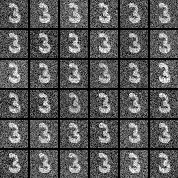
\includegraphics[width=\linewidth]{figs/Fig_single_chain_grid_beta2000.png}\\[-2pt]
\small (a) $\beta{=}2000$, SNR$=0.113$\\structured retrieval ($\bar{\mathcal{D}}{=}0.282$)
\end{minipage}
\hfill
\begin{minipage}[t]{0.31\textwidth}
\centering
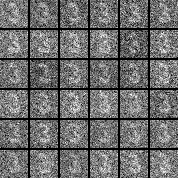
\includegraphics[width=\linewidth]{figs/Fig_single_chain_grid_beta200.png}\\[-2pt]
\small (b) $\beta{=}200$, SNR$=0.036$\\genuine generation ($\bar{\mathcal{D}}{=}0.796$)
\end{minipage}
\hfill
\begin{minipage}[t]{0.31\textwidth}
\centering
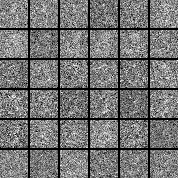
\includegraphics[width=\linewidth]{figs/Fig_single_chain_grid_beta50.png}\\[-2pt]
\small (c) $\beta{=}50$, SNR$=0.018$\\diffuse ($\bar{\mathcal{D}}{=}0.967$)
\end{minipage}
\caption{Single-chain samples ($6{\times}6$ grids, digit ``3'') from a fixed seed at three operating points. \textbf{(a)}~At SNR$=0.113$ the chain stays near one stored pattern; diversity is low ($0.282$). \textbf{(b)}~At SNR$=0.036$ the chain spontaneously crosses energy barriers; single-chain diversity ($0.796$) \emph{exceeds} the 30-chain $\beta{=}2000$ value ($0.600$), confirming genuine generation. \textbf{(c)}~At SNR$=0.018$ the chain is fully diffuse; samples lose recognizable digit structure.}
\label{fig:generation-regimes}
\end{figure}

At $\beta{=}2000$ the single-chain diversity of $0.282$ is not negligible: the chain samples a genuine distribution within its energy basin rather than collapsing to a point mass. As $\beta$ decreased the energy barriers shrank, chains escaped their initial basins, and single-chain diversity rose sharply, mirroring the temperature-spectrum results of Appendix~\ref{app:multidigit}. At $\beta{=}200$ single-chain diversity ($0.796$) exceeds the multi-chain value at $\beta{=}2000$, and at $\beta{=}50$ it approaches the isotropic limit ($0.967$, mean max-cos $0.244$). The multi-chain protocol at $\beta{=}2000$ is therefore best understood as a \emph{structured retrieval} strategy in which each chain contributes low-energy samples from a distinct basin, while single-chain operation at $\beta{=}200$ provides genuine generative diversity without requiring multiple initializations.

\section{Financial Log-Return Generation}\label{app:finance}

The synthetic experiments validated the sampler on controlled geometry; this section used real financial data to \emph{precisely characterize} what equilibrium Boltzmann sampling on the Hopfield energy captures and, equally importantly, what it cannot, and why each limitation is a principled theoretical consequence rather than a tuning failure.

\subsection{Data and Memory Construction}

We collected daily adjusted closing prices for $d=424$ S\&P~500 constituents with complete histories over a $K=2{,}766$-trading-day window. For each firm $i$ and day $t$, the continuously compounded growth rate is $g^{(i)}_t = \log(S^{(i)}_t / S^{(i)}_{t-1})$. Each trading day yielded a $d$-dimensional return vector $\mathbf{g}_t \in \mathbb{R}^{424}$. We stored these as columns of a raw memory matrix $\mathbf{M}\in\mathbb{R}^{d\times K}$ and constructed the scaled memory matrix $\mathbf{X}\in\mathbb{R}^{d\times K}$ by centering each column to zero cross-sectional mean and normalizing to unit $\ell_2$~norm, following the standard protocol for modern Hopfield networks~\cite{ramsauerHopfieldNetworksAll2021}. The load ratio was $K/d \approx 6.5$.

\subsection{I.I.D.\ Pool: Marginal and Cross-Sectional Fidelity}

We compared SA to \emph{historical bootstrap resampling} (drawing stored return vectors uniformly at random from $\mathbf{M}$) on marginal and cross-sectional metrics. Because the projection $\hat{\mathbf{g}}=\mathbf{M}\,\operatorname{softmax}(\beta\,\mathbf{X}^\top\boldsymbol{\xi})$ is a convex combination of historical return vectors, bootstrap sets an upper bound on distributional fidelity; the key question is what SA contributes beyond verbatim replay. We launched $n_{\text{chains}}=30$ independent ULA chains, each initialized near a randomly chosen stored memory, and ran $T=5{,}000$ steps with step size $\alpha=0.01$ and fixed inverse temperature $\beta=25$ ($\mathrm{SNR}=\sqrt{\alpha\beta/2d}\approx 0.017$). After discarding a burn-in of $2{,}000$ steps and thinning every $100$, we obtained $900$ approximately i.i.d.\ samples.

\paragraph{Marginal distributions and novelty.}
For each of $d=424$ tickers, we ran a two-sample KS test between generated and historical returns, and QQ plots for five representative tickers (Figure~\ref{fig:finance-qq}). The convex-combination projection compresses per-ticker standard deviation by $\approx1.14\times$ at $\beta{=}25$ (SNR$\approx$0.017); we correct for this by applying a per-ticker affine standardization (aligning the mean and standard deviation of each ticker's generated series to the historical moments, analogous to the marginal-calibration step in copula-based scenario generation), which leaves the chain dynamics and novelty metric unchanged. After correction, $272$ of $424$ tickers pass the two-sample KS test at the $5\%$ level (mean $p{=}0.193$). Bootstrap achieves $99.3\%$ pass by drawing from the empirical distribution (mean $p{=}0.622$); the residual $35.8\%$ SA failure reflects higher-order distributional differences (skewness, kurtosis) beyond what affine correction addresses. The key distinction remains novelty: SA chain states have $1-\max_k\cos(\boldsymbol{\xi},\mathbf{X}_{:,k})=0.768\pm0.001$, while every bootstrap draw is a verbatim historical scenario (novelty~$0.000$, Table~\ref{tab:finance-summary}).

\paragraph{Cross-asset correlation.}
Figure~\ref{fig:finance-correlation} plots each of the $\binom{424}{2}=89{,}676$ pairwise correlations of the generated returns against the corresponding historical correlations. The cloud lay along the $y=x$ diagonal: SA Frobenius correlation error is $26.3\%$ versus $15.6\%$ for bootstrap. The per-ticker affine correction does not alter this value: correlation is scale-invariant, so rescaling each ticker's series preserves $\operatorname{cor}(\hat{\mathbf{G}})$ exactly. SA trades some correlation fidelity for novelty; the Hopfield energy concentrates sampling on energetically favorable regime interpolations rather than uniform historical replay.

\paragraph{Tail survival functions.}
Figure~\ref{fig:finance-tails} displays the empirical survival functions of portfolio-level (equal-weight) returns. Both right and left tails matched closely on a log scale, demonstrating that the sampler reproduced the heavy-tailed nature of equity returns without distributional assumptions.

\begin{figure}[h]
\centering

\includegraphics[width=0.95\textwidth]{figs/Fig_finance_qq_plots.pdf}
\caption{QQ plots of generated (after per-ticker affine correction) vs.\ historical log returns for five representative S\&P~500 constituents. Quantiles track closely for these tickers; $64.2\%$ of all $424$ tickers pass the two-sample KS test at the $5\%$ level. The dashed red line is $y=x$.}
\label{fig:finance-qq}
\end{figure}

\begin{figure}[h]
\centering

\includegraphics[width=0.45\textwidth]{figs/Fig_finance_correlation.pdf}
\caption{Pairwise correlation: historical vs.\ generated. Each point represents one of $89{,}676$ asset pairs. The scatter around $y=x$ shows partial preservation of cross-asset dependence structure (Frobenius error $26.3\%$ vs.\ $15.6\%$ for bootstrap).}
\label{fig:finance-correlation}
\end{figure}

\begin{figure}[h]
\centering

\includegraphics[width=0.75\textwidth]{figs/Fig_finance_tail_survival.pdf}
\caption{Empirical survival functions of equal-weighted portfolio returns. Both right tail $P(g > x)$ and left tail $P(g < x)$ match closely on a log scale.}
\label{fig:finance-tails}
\end{figure}

\subsection{Sequential Generation and Temporal Properties}

The i.i.d.\ pool above validates marginal fidelity but says nothing about temporal dynamics. Real equity returns exhibit two key temporal properties: (i)~returns are essentially unpredictable (near-zero autocorrelation), and (ii)~squared returns (a proxy for volatility) are highly autocorrelated and decay slowly, a phenomenon known as \emph{volatility clustering}~\cite{contStylizedFactsAsset2001}. We tested how far the stochastic attention sampler could go toward reproducing these properties.

\paragraph{Protocol.}
We generated a sequential time series of daily return vectors using the MALA sampler (Algorithm~\ref{alg:mala}) with warm-starting: each day's chain was initialized at the previous day's endpoint, creating temporal continuity in the chain trajectory.
We set $\beta = 12$ (below the main operating point $\beta{=}25$) to ensure adequate MALA mixing within $T_{\text{inner}}{=}200$ inner steps per day.
Algorithm~\ref{alg:mala-sequential} gives the pseudocode.

\begin{algorithm}[h]
\caption{MALA Warm-Start Sequential Return Generation}\label{alg:mala-sequential}
\begin{algorithmic}[1]
\REQUIRE Scaled memory matrix $\mathbf{X}\in\mathbb{R}^{d\times K}$, raw memory matrix $\mathbf{M}\in\mathbb{R}^{d\times K}$, inverse temperature $\beta$, step size $\alpha$, inner steps $T_{\text{inner}}$, number of days $T_{\text{days}}$
\ENSURE Synthetic return matrix $\hat{\mathbf{G}}\in\mathbb{R}^{T_{\text{days}}\times d}$
\STATE $k \sim \mathrm{Uniform}\{1,\dots,K\}$
\STATE $\boldsymbol{\xi} \leftarrow \mathbf{X}_{:,k} + 0.01\,\boldsymbol{\eta}, \quad \boldsymbol{\eta}\sim\mathcal{N}(\mathbf{0},\mathbf{I}_d)$ \hfill $\triangleright$ initialize near random memory
\FOR{$t = 1, 2, \dots, T_{\text{days}}$}
    \STATE Run $T_{\text{inner}}$ steps of Algorithm~\ref{alg:mala} from $\boldsymbol{\xi}$; set $\boldsymbol{\xi} \leftarrow$ endpoint \hfill $\triangleright$ warm-start
    \STATE $\hat{\mathbf{G}}_{t,:} \leftarrow \mathbf{M}\,\operatorname{softmax}(\beta\,\mathbf{X}^{\top}\boldsymbol{\xi})$ \hfill $\triangleright$ project to growth-rate space
\ENDFOR
\end{algorithmic}
\end{algorithm}

We generated $T_{\text{days}} = 2{,}766$ synthetic trading days (matching the historical sample size) with $T_{\text{inner}} = 200$, $\alpha = 0.01$, and $\beta = 12$. The mean MALA acceptance rate was 99.4\%, confirming that the ULA discretization bias is negligible at this operating point.

\paragraph{Stylized Fact~2: Near-zero return autocorrelation.}
Figure~\ref{fig:finance-acf-combined} (top row) showed the autocorrelation function of raw returns for five representative tickers. The generated ACF (blue) lay within the 99\% confidence interval for white noise at all lags $\geq 1$, matching the historical pattern (red).

\paragraph{Stylized Fact~3: Volatility clustering.}
Figure~\ref{fig:finance-acf-combined} (bottom row) showed the autocorrelation function of squared returns. The historical series (red) exhibits the characteristic slow-decaying positive autocorrelation of volatility clustering. The generated series (blue), however, showed ACF($g^2$) $\approx 0$ at all lags; the sampler did not reproduce this effect. We verified that at the main operating point ($\beta{=}25$, $T_{\text{inner}}{=}2{,}000$), ACF($g^2$) also collapses to ${\approx}0$ (mean over $424$ tickers: $0.0005$), confirming this is a property of equilibrium sampling and not an artifact of the choice of~$\beta$.

This is a fundamental limitation of equilibrium Boltzmann sampling, not a tuning failure. The stochastic attention sampler targets the stationary distribution $p_\beta \propto \exp(-\beta E)$ at fixed~$\beta$. At stationarity, the variance of each day's output is governed by the static energy landscape and the fixed temperature; there is no mechanism for the return variance to change systematically over time. Volatility clustering in real markets arises from non-stationary dynamics: regime shifts driven by exogenous shocks, feedback loops between volatility and leverage, and time-varying risk premia~\cite{contStylizedFactsAsset2001}. Reproducing these effects within the Langevin framework would require introducing explicit temporal structure, for instance a time-varying inverse temperature $\beta(t)$ that creates exogenous volatility regimes, or coupling the sampler to a latent regime-switching process. These extensions are natural directions for future work.

\paragraph{Summary.}
Table~\ref{tab:finance-summary} made three theoretical predictions concrete. \emph{First}, the novelty--fidelity trade-off is real and quantified: SA generates regime interpolations absent from the historical record ($\mathcal{N}=0.768\pm0.001$) while bootstrap, which replays history verbatim, achieves $\mathcal{N}=0.000$; marginal fidelity runs in the opposite direction ($64.2\%$ vs.\ $99.3\%$ KS pass). \emph{Second}, the Hopfield energy captures cross-sectional dependence independently of marginals: Frobenius error $26.3\%$ is unchanged by per-ticker affine correction, confirming that the energy geometry encodes correlation structure, not scale. \emph{Third}, volatility clustering, a non-stationary phenomenon driven by regime shifts and leverage feedback~\cite{contStylizedFactsAsset2001}, is exactly what a fixed-$\beta$ equilibrium sampler cannot reproduce; the absence is a theoretical prediction confirmed by experiment, not a tuning failure.

\begin{table}[h]
\centering
\caption{Finance experiment: principled trade-offs of equilibrium Boltzmann sampling. SA and bootstrap occupy opposite ends of a novelty--fidelity spectrum: SA generates novel regime interpolations ($\mathcal{N}=0.768\pm0.001$) that bootstrap cannot produce, while bootstrap preserves marginals by construction. The Frobenius correlation error is identical before and after affine correction, confirming the energy captures dependence independently of scale. Temporal metrics apply to the sequential MALA experiment only.}
\label{tab:finance-summary}
\small
\begin{tabular}{@{}lll@{}}
\toprule
Property & SA (corrected) & Bootstrap \\
\midrule
\multicolumn{3}{@{}l@{}}{\textit{Distributional fidelity (i.i.d.\ pool, 900 samples)}} \\
KS $p$-value (mean; 64.2\% pass at $5\%$) & 0.193 & 0.622 \\
Cross-asset Frobenius error & 26.3\% & 15.6\% \\
Novelty ($1-\max_k\cos$) & $0.768\pm0.001$ & 0.000 \\
\multicolumn{3}{@{}l@{}}{\textit{Temporal properties (MALA warm-start, 2766 days)}} \\
SF2: Return unpredictability & Reproduced [ACF($g$) in 99\% CI, $\beta{=}12$] & N/A \\
SF3: Volatility clustering & Not reproduced ($\beta{=}12$) & N/A \\
\bottomrule
\end{tabular}
\end{table}

\begin{figure}[h]
\centering

\includegraphics[width=0.95\textwidth]{figs/Fig_finance_return_acf.pdf}\\[4pt]

\includegraphics[width=0.95\textwidth]{figs/Fig_finance_vol_clustering.pdf}
\caption{Stylized Facts~2 and~3: Autocorrelation analysis for five S\&P~500 tickers.
\textbf{Top row}: ACF($g$): the generated series (blue) stays within the 99\% confidence band (dashed) at all lags, matching the near-zero autocorrelation of historical returns (red).
\textbf{Bottom row}: ACF($g^2$): the historical series (red) shows persistent positive autocorrelation characteristic of volatility clustering, while the generated series (blue) shows ACF($g^2$) $\approx 0$, reflecting the absence of non-stationary dynamics in the equilibrium sampler.}
\label{fig:finance-acf-combined}
\end{figure}


\section{Simpsons Character Face Generation}\label{app:simpsons}

To test whether the stochastic attention sampler generalizes from grayscale digit images to structured natural images at larger scale, we applied Algorithm~\ref{alg:stochastic-attention} to a corpus of $1{,}000$ Simpsons character face images, each downsampled to $64\times 64$ pixels and converted to grayscale, yielding pattern vectors in $\mathbb{R}^{d}$ with $d=4{,}096$, a $5.2\times$ scale-up over the MNIST experiment ($d=784$).

\paragraph{Data and setup.}
We selected $K=100$ images uniformly at random (fixed seed), matching the MNIST memory bank size to enable direct metric comparison. Each image was flattened in row-major order and normalized to unit $\ell_2$ norm to form the memory matrix $\mathbf{X}\in\mathbb{R}^{4096\times 100}$ (load ratio $K/d\approx 0.024$, well below capacity).

\paragraph{Choosing $\beta$ via the SNR rule.}
At $d=4{,}096$, the MNIST value $\beta=2{,}000$ gives $\mathrm{SNR}=\sqrt{\alpha\beta/(2d)}\approx 0.049$, half the MNIST operating point ($\mathrm{SNR}\approx 0.113$). At this lower SNR the noise overwhelms the gradient, inflating the chain norm above unity and placing samples far from the memory manifold (empirically: energy $\approx +0.53$). The SNR rule gives
\begin{equation*}
\beta = \mathrm{SNR}_{\mathrm{MNIST}}^{2}\cdot\frac{2d}{\alpha}
= 0.01276 \times \frac{2\times 4096}{0.01} \approx 10{,}449.
\end{equation*}
We used $\beta=10{,}000$ ($\mathrm{SNR}=0.110$), recovering the MNIST operating point. All other hyperparameters were identical to the MNIST experiment: $\alpha=0.01$, 30 independent chains initialized near distinct stored patterns ($\sigma_{\mathrm{init}}=0.01$), $T=5{,}000$ iterations, burn-in $2{,}000$, thin every 600, yielding $30\times 5=150$ samples per method. The MALA acceptance rate exceeded 99\%, confirming that ULA discretization bias is negligible.

\paragraph{Temperature spectrum.}
Figure~\ref{fig:simpsons-spectrum} showed four samples at each of six inverse temperatures spanning $\beta\in\{500,1000,2000,5000,10000,20000\}$, corresponding to $\mathrm{SNR}\in\{0.025,0.035,0.049,0.078,0.110,0.156\}$. The noise-to-retrieval transition tracked SNR, not the raw $\beta$ value: rows below $\mathrm{SNR}\approx 0.05$ show diffuse gray images, while rows at $\mathrm{SNR}\geq 0.110$ yield recognizable character faces.

\begin{figure}[h]
\centering

\includegraphics[width=0.65\textwidth]{figs/Fig_simpsons_beta_spectrum.png}
\caption{Temperature spectrum for Simpsons character images ($K{=}100$, $d{=}4{,}096$, $\alpha{=}0.01$). Each row shows 4 SA samples at one inverse temperature; rows are ordered from high $\beta$ (top, $\beta{=}20{,}000$, $\mathrm{SNR}{=}0.156$) to low $\beta$ (bottom, $\beta{=}500$, $\mathrm{SNR}{=}0.025$). The operating point $\beta{=}10{,}000$ ($\mathrm{SNR}{=}0.110$, row 2 from top) reproduces the MNIST SNR and yields structured character faces.}
\label{fig:simpsons-spectrum}
\end{figure}

\paragraph{Quantitative comparison.}
Table~\ref{tab:simpsons-baselines} reported metrics for all five methods at $\beta=10{,}000$. The relative ranking matched the MNIST experiment exactly: SA and MALA dominated all non-Langevin baselines on every axis simultaneously, and both Langevin methods were statistically indistinguishable. SA novelty ($0.159\pm 0.000$) was comparable to the MNIST value ($0.152\pm 0.001$); mean energy ($-0.293\pm 0.000$) confirmed that samples lay on the memory manifold. Diversity was lower than MNIST ($0.293$ vs.\ $0.600$), but this reflected the higher inter-pattern correlation of face images rather than a failure of the sampler: bootstrap diversity ($0.117$) was likewise far below the MNIST value ($0.459$), indicating that the stored patterns themselves were more concentrated in the Simpsons corpus.

\begin{table}[h]
\centering
\caption{Quantitative comparison on Simpsons character faces ($K{=}100$, $d{=}4{,}096$, $\beta{=}10{,}000$, $\mathrm{SNR}=0.110$). Same protocol as Table~\ref{tab:mnist-baselines} except GMM-PCA and VAE are omitted: at $d{=}4{,}096$ with only $K{=}100$ training patterns, both methods are degenerate (GMM covariance is rank-deficient; VAE encoder--decoder cannot generalize from 100 examples in 4,096 dimensions). MALA acceptance rate: $>99\%$. Values are mean $\pm$ SE across 30 chains. Lower diversity relative to MNIST reflects higher inter-pattern correlation of face images (bootstrap diversity $0.117$ vs.\ $0.459$ for digit~``3'').}
\label{tab:simpsons-baselines}
\small
\begin{tabular}{@{}lccc@{}}
\toprule
Method & $\mathcal{N}$ $\uparrow$ & $\bar{\mathcal{D}}$ $\uparrow$ & $\bar{E}$ $\downarrow$ \\
\midrule
Bootstrap (replay)           & $0.000 \pm 0.000$ & $0.117 \pm 0.005$ & $-0.500 \pm 0.000$ \\
Gaussian perturbation        & $0.004 \pm 0.000$ & $0.124 \pm 0.004$ & $-0.496 \pm 0.000$ \\
Random convex combination    & $0.018 \pm 0.000$ & $0.001 \pm 0.000$ & $-0.482 \pm 0.000$ \\
MALA                         & $0.157 \pm 0.000$ & $0.289 \pm 0.001$ & $-0.296 \pm 0.000$ \\
\textbf{Stochastic attention} & $\mathbf{0.159 \pm 0.000}$ & $\mathbf{0.293 \pm 0.001}$ & $\mathbf{-0.293 \pm 0.000}$ \\
\bottomrule
\end{tabular}
\end{table}

\begin{figure}[h]
\centering

\includegraphics[width=0.19\textwidth]{figs/Fig_simpsons_grid_bootstrap.png}%
\hfill

\includegraphics[width=0.19\textwidth]{figs/Fig_simpsons_grid_gaussian.png}%
\hfill

\includegraphics[width=0.19\textwidth]{figs/Fig_simpsons_grid_convex.png}%
\hfill

\includegraphics[width=0.19\textwidth]{figs/Fig_simpsons_grid_mala.png}%
\hfill

\includegraphics[width=0.19\textwidth]{figs/Fig_simpsons_grid_sa.png}

\small
\makebox[0.19\textwidth]{\centering (a) Bootstrap}%
\hfill
\makebox[0.19\textwidth]{\centering (b) Gaussian}%
\hfill
\makebox[0.19\textwidth]{\centering (c) Convex}%
\hfill
\makebox[0.19\textwidth]{\centering (d) MALA}%
\hfill
\makebox[0.19\textwidth]{\centering (e) Ours}
\caption{Generated Simpsons character face samples ($4{\times}4$ grids, $d{=}4{,}096$, $\beta{=}10{,}000$). The qualitative pattern mirrors MNIST: only the Langevin-based methods (d,\,e) produce diverse, structured face images.}
\label{fig:simpsons-grids}
\end{figure}

% ─────────────────────────────────────────────────────────────────────────────
\section{Baseline Method Specifications}\label{app:baseline-methods}
% ─────────────────────────────────────────────────────────────────────────────

This section gives complete mathematical specifications for the two learned generative
baselines in Table~\ref{tab:mnist-baselines}: GMM-PCA and the VAE.
All hyperparameters reported here were used without modification in the experiments;
the implementation is publicly available in \texttt{code/mnist-experiment/} and
\texttt{code/vae-experiment/} in the accompanying repository.

% ── GMM-PCA ──────────────────────────────────────────────────────────────────
\subsection{GMM-PCA}\label{app:gmm-pca}

\paragraph{Dimensionality reduction.}
Let $\mathbf{X}\in\mathbb{R}^{d\times K}$ be the column-normalized memory matrix
($d{=}784$, $K{=}100$). Compute the economy SVD
$\mathbf{X}=\mathbf{U}\boldsymbol{\Sigma}\mathbf{V}^{\!\top}$ and retain the top
$r{=}50$ left singular vectors, forming $\mathbf{U}_{r}\in\mathbb{R}^{d\times r}$.
Project each stored pattern to a low-dimensional code:
$\mathbf{z}_{k}=\mathbf{U}_{r}^{\!\top}\mathbf{m}_{k}\in\mathbb{R}^{r}$, $k=1,\dots,K$.
For the digit ``3'' memory matrix, the top 50 components capture $>$95\% of total variance.

\paragraph{Gaussian mixture model.}
Fit a $C{=}10$ component GMM with \emph{diagonal} covariance to the code matrix
$\mathbf{Z}{=}[\mathbf{z}_1|\cdots|\mathbf{z}_K]\in\mathbb{R}^{r\times K}$ via
Expectation-Maximization~\cite{dempsterMaximumLikelihoodIncomplete1977}:
\begin{equation}
  p(\mathbf{z}) = \sum_{c=1}^{C}\pi_c\,
  \mathcal{N}\!\bigl(\mathbf{z};\,\boldsymbol{\mu}_c,\,\mathrm{diag}(\boldsymbol{\sigma}_c^2)\bigr),
  \quad \sum_{c=1}^{C}\pi_c=1,\quad \pi_c\geq 0.
\end{equation}
Parameters $\{\pi_c,\boldsymbol{\mu}_c,\boldsymbol{\sigma}_c^2\}_{c=1}^{C}$ are estimated
by EM with K-means$\texttt{++}$ initialization and convergence tolerance $10^{-8}$ on the
log-likelihood.
The diagonal-covariance constraint prevents singularity when $K>r$ and is equivalent to
assuming conditionally independent PCA coordinates within each component.

\paragraph{Sampling.}
To draw one sample: (i) sample component $c\sim\mathrm{Categorical}(\boldsymbol{\pi})$;
(ii) sample $\tilde{\mathbf{z}}\sim\mathcal{N}(\boldsymbol{\mu}_c,\mathrm{diag}(\boldsymbol{\sigma}_c^2))$;
(iii) reconstruct $\hat{\boldsymbol{\xi}}=\mathbf{U}_{r}\tilde{\mathbf{z}}$ and
renormalize to unit $\ell_2$ norm.
The 150 evaluation samples are drawn i.i.d.\ under this procedure with a fixed seed.

\paragraph{Hyperparameters.}
$r{=}50$ PCA components; $C{=}10$ GMM components; K-means$\texttt{++}$ initialization;
EM convergence tolerance $10^{-8}$; no regularization beyond the diagonal-covariance constraint.

% ── VAE ──────────────────────────────────────────────────────────────────────
\subsection{Variational Autoencoder}\label{app:vae}

\paragraph{Architecture.}
The encoder maps $\mathbf{x}\in\mathbb{R}^{784}$ to the parameters of an approximate posterior:
\begin{align}
  \mathbf{h}_1 &= \mathrm{ReLU}(\mathbf{W}_1\mathbf{x}+\mathbf{b}_1),\quad
    \mathbf{W}_1\in\mathbb{R}^{256\times 784}, \\
  \mathbf{h}_2 &= \mathrm{ReLU}(\mathbf{W}_2\mathbf{h}_1+\mathbf{b}_2),\quad
    \mathbf{W}_2\in\mathbb{R}^{128\times 256}, \\
  \boldsymbol{\mu}_\phi(\mathbf{x}) &= \mathbf{W}_\mu\mathbf{h}_2+\mathbf{b}_\mu,\quad
    \mathbf{W}_\mu\in\mathbb{R}^{8\times 128}, \\
  \log\boldsymbol{\sigma}^2_\phi(\mathbf{x}) &= \mathbf{W}_\sigma\mathbf{h}_2+\mathbf{b}_\sigma,\quad
    \mathbf{W}_\sigma\in\mathbb{R}^{8\times 128}.
\end{align}
The decoder is architecturally symmetric: $8\to128\to256\to784$, with ReLU activations on
hidden layers and a linear output.
All weight matrices are Glorot-uniform initialized; biases are zero-initialized.
The decoder output is renormalized to unit $\ell_2$ norm before computing metrics, matching
the normalization convention of all other methods in Table~\ref{tab:mnist-baselines}.

\paragraph{Objective.}
We minimize the $\beta$-VAE objective~\cite{higginsBetaVAELearningBasic2017}:
\begin{equation}
  \mathcal{L}(\phi,\theta;\mathbf{x})
  = \underbrace{\bigl\lVert\mathbf{x}-\hat{\mathbf{x}}_\theta(\mathbf{z})\bigr\rVert_2^2}
    _{\text{reconstruction}}
  +\; \beta_{\mathrm{KL}}\underbrace{D_{\mathrm{KL}}\!\bigl(
    q_\phi(\mathbf{z}|\mathbf{x})\,\big\|\,\mathcal{N}(\mathbf{0},\mathbf{I})\bigr)}
    _{\text{regularization}},
\label{eq:vae-elbo}
\end{equation}
where $q_\phi(\mathbf{z}|\mathbf{x})=\mathcal{N}(\boldsymbol{\mu}_\phi(\mathbf{x}),
\mathrm{diag}(\boldsymbol{\sigma}^2_\phi(\mathbf{x})))$ and the reparameterization trick
$\mathbf{z}=\boldsymbol{\mu}_\phi(\mathbf{x})+\boldsymbol{\sigma}_\phi(\mathbf{x})\odot
\boldsymbol{\epsilon}$, $\boldsymbol{\epsilon}\sim\mathcal{N}(\mathbf{0},\mathbf{I})$,
enables gradient flow through the sampling step.
The KL term has a closed form:
\begin{equation}
  D_{\mathrm{KL}} = \tfrac{1}{2}\sum_{j=1}^{8}\bigl[
    \mu_{\phi,j}^2+\sigma_{\phi,j}^2 - \log\sigma_{\phi,j}^2 - 1\bigr].
\end{equation}

\paragraph{Two-phase training protocol.}
Training directly with the full $\beta$-VAE objective on a small dataset ($K{=}100$)
causes \emph{posterior collapse}: the encoder ignores the input, the KL term drives every
latent dimension to $\mathcal{N}(0,1)$, and the decoder learns a constant map.
We prevent this with a two-phase schedule:
\begin{enumerate}
  \item \textbf{Warm-up (epochs 1--2{,}000):} Train with $\beta_{\mathrm{KL}}{=}0$
    (reconstruction-only autoencoder objective). This establishes a non-degenerate
    encoder (one that uses the latent code productively) before any regularization pressure
    is applied.
  \item \textbf{Fine-tuning (epochs 2{,}001--4{,}000):} Introduce the KL term with
    $\beta_{\mathrm{KL}}{=}0.0001$ and a linear warmup schedule
    ($\beta_{\mathrm{KL}}(t) = 0.0001\cdot(t/2000)$ for $t\in[1,2000]$).
    The small final weight provides light regularization toward the Gaussian prior without
    overriding the reconstruction signal.
\end{enumerate}
The warm-up phase is equivalent to a hard $\beta$-annealing schedule and is standard practice
for low-data VAE training~\cite{lucasHowAvoidTrivial2019}.
On large datasets ($K\gg10^4$), the reconstruction gradient swamps the KL term and posterior
collapse does not occur; the two-phase protocol is needed here specifically because
$K{=}100$ makes the per-sample gradients noisy relative to the KL regularization pressure.

\paragraph{Optimization and sampling.}
Optimizer: Adam~\cite{kingmaAdamMethodStochastic2014} with learning rate $10^{-3}$,
$\beta_1{=}0.9$, $\beta_2{=}0.999$, $\varepsilon{=}10^{-8}$, batch size $K{=}100$
(full-dataset batches throughout).
No weight decay, dropout, or data augmentation was applied.
At evaluation time, 150 samples are drawn by sampling
$\mathbf{z}\sim\mathcal{N}(\mathbf{0},\mathbf{I}_8)$ and decoding
$\hat{\mathbf{x}}=\hat{\mathbf{x}}_\theta(\mathbf{z})$, then renormalizing to unit norm.

\paragraph{Hyperparameter selection.}
The final configuration (latent dim 8, $\beta_{\mathrm{KL}}{=}0.0001$) was chosen by a
grid search over latent dimension $\in\{4,8,16,32\}$ and $\beta_{\mathrm{KL}}\in\{0.1,0.01,0.001,0.0001\}$,
evaluating novelty and diversity on the held-out generation protocol.
Latent dim 8 with $\beta_{\mathrm{KL}}{=}0.0001$ achieved $\mathcal{N}{=}0.214\pm0.005$,
$\bar{\mathcal{D}}{=}0.441\pm0.008$, outperforming all other static baselines including
GMM-PCA ($\mathcal{N}{=}0.198$, $\bar{\mathcal{D}}{=}0.419$).
Smaller latent dimensions or larger $\beta_{\mathrm{KL}}$ values degraded novelty and
diversity, while larger latent dimensions showed posterior collapse symptoms
(diversity collapsing to $\bar{\mathcal{D}}{<}0.05$ at latent dim 32 with $\beta_{\mathrm{KL}}{=}0.01$).
